%-----------------------------------------------%
% abnTeX2: Modelo de Trabalho Academico em conformidade com 
% ABNT NBR 14724:2011: Informacao e documentacao - Trabalhos academicos -
% Apresentacao
%
% Adaptado por Rodrigo Nascimento (2022-08-12) modelo baseado no 
% https://github.com/emersonmello/modelos-latex/tree/master/monografia
% criado pelo professor Emerson Mello (IFSC)
%-----------------------------------------------%

\documentclass[
	% -- opções da classe memoir --
	12pt,				% tamanho da fonte
	openright,			% capítulos começam em pág ímpar (insere página vazia caso preciso)
	oneside,			% twoside para impressão em verso e anverso. Oposto a oneside
	a4paper,			% tamanho do papel. 
	% -- opções da classe abntex2 --
	chapter=TITLE,		% títulos de capítulos convertidos em letras maiúsculas
	%section=TITLE,		% títulos de seções convertidos em letras maiúsculas
	%subsection=TITLE,	% títulos de subseções convertidos em letras maiúsculas
	%subsubsection=TITLE,% títulos de subsubseções convertidos em letras maiúsculas
	% -- opções do pacote babel --
	english,			% idioma adicional para hifenização
%	french,				% idioma adicional para hifenização
%	spanish,			% idioma adicional para hifenização
	brazil				% o último idioma é o principal do documento
]{abntex2}

%-----------------------------------------------%
% Informações de dados para CAPA e FOLHA DE ROSTO
%-----------------------------------------------%
\instituicao{Universidade do Estado de Santa Catarina -- UDESC}
\titulo{Estágio Curricular Supervisionado -- III}
\autor{Rodrigo Ribamar Silva do Nascimento}
\local{Joinville - SC}
\data{Agosto/2022}
\tipotrabalho{Relatório}
\orientador{Prof. Dr. Carlos R. Rocha Zorack}
\coorientador{Prof. Me. Mário Heleno Calegari}
%-----------------------------------------------%
% Para alterar o parâmetros dos comandos orientador
% e coorientador.
%-----------------------------------------------%
% \renewcommand{\orientadorname}{Orientadora:}
\renewcommand{\coorientadorname}{Supervisor:}
%-----------------------------------------------%

\newcommand{\centro}{Centro de Ciências Tecnológicas -- CCT }
\newcommand{\departamento}{Departamento de Física -- DFIS}
\newcommand{\curso}{Licenciatura em Física }
\newcommand{\disciplina}{Estágio Curricular Supervisionado III -- ESC3003}
\newcommand{\firstkey}{Estágio Supervisionado}
\newcommand{\secondkey}{Ensino de Física}
\newcommand{\thirdkey}{Docência Compartilhada}


%-----------------------------------------------%

% Todas as indicações de pacotes e configurações estão no arquivo de estilo
% chamado texmodel-udesc.sty.
\usepackage{texmodel-udesc}

%-----------------------------------------------%
% Estilo de cabeçalho que só contém o número da 
% página e uma linha
%-----------------------------------------------%
\makepagestyle{cabecalholimpo}
\makeevenhead{cabecalholimpo}{\thepage}{}{} % páginas pares
\makeoddhead{cabecalholimpo}{}{}{\thepage} % páginas ímpares
%\makeheadrule{cabecalholimpo}{\textwidth}{\normalrulethickness} % linha
%-----------------------------------------------%

%-----------------------------------------------%
% Início do documento
%-----------------------------------------------%
\begin{document}

% Seleciona o idioma do documento (conforme pacotes do babel)
\selectlanguage{brazil}
% Retira espaço extra obsoleto entre as frases.
\frenchspacing
%-----------------------------------------------%
% ELEMENTOS PRÉ-TEXTUAIS
%-----------------------------------------------%
\pretextual
\imprimircapa
%-----------------------------------------------%
% No arquivo abaixo tem detalhes sobre folha de
% aprovação, ficha catalográfica, agradecimentos,
% resumo, abstract, etc.
% 
% Se não for a versão final do PDF, talvez fosse
% interessante comentar a linha abaixo.
%-----------------------------------------------%
% Folha de rosto - (o * indica que haverá a ficha bibliográfica)

%-----------------------------------------------%
% ARQUIVOS PRETEXTUAIS
% ----------------------------------------------%
\imprimirfolhaderosto*

%\includepdf{aprovacao.pdf}
%-----------------------------------------------%
% Inserir a ficha bibliografica %
%-----------------------------------------------%
% Isto é um exemplo de Ficha Catalográfica, ou ``Dados internacionais de
% catalogação-na-publicação''. Você pode utilizar este modelo como referência. 
% Porém, provavelmente a biblioteca da sua universidade lhe fornecerá um PDF
% com a ficha catalográfica definitiva após a defesa do trabalho. Quando estiver
% com o documento, salve-o como PDF no diretório do seu projeto e substitua todo
% o conteúdo de implementação deste arquivo pelo comando abaixo:
%
% \begin{fichacatalografica}
%     %\includepdf{fig_ficha_catalografica.pdf}    
% \end{fichacatalografica}

% ------------------------------
%EXEMPLO DE FICHA CATALOGRÁFICA
% ------------------------------
% \begin{fichacatalografica}
% 	\sffamily
% 	\vspace*{\fill}					% Posição vertical
% 	\begin{center}					% Minipage Centralizado
%         \fbox{
%             \begin{minipage}[c][8cm]{13.5cm}		% Largura
%                 \small
%                 \imprimirautor
%                 %Sobrenome, Nome do autor
                
%                 \hspace{0.5cm} \imprimirtitulo  / \imprimirautor. --
%                 \imprimirlocal, \imprimirdata-
                
%                 \hspace{0.5cm} \pageref{LastPage} p. : il. (algumas color.) ; 30 cm.\\
                
%                 \hspace{0.5cm} \imprimirorientadorRotulo~\imprimirorientador\\
                
%                 \hspace{0.5cm}
%                 \parbox[t]{\textwidth}{\imprimirtipotrabalho~--~\imprimirinstituicao,
%                 \imprimirdata.}\\
                
%                 \hspace{0.5cm}
%                     1. \firstkey.
%                     2. \secondkey.
%                     2. \thirdkey.
%                     I. Orientador.
%                     II. Universidade do Estado de Santa Catarina.
%                     III. \centro.
%                     IV. Título.
%             \end{minipage}
%         }
% 	\end{center}
% \end{fichacatalografica}
%-----------------------------------------------%

%-----------------------------------------------%
% Inserir folha de aprovação
%-----------------------------------------------%

% Isto é um exemplo de Folha de aprovação, elemento obrigatório da NBR
% 14724/2011 (seção 4.2.1.3). Você pode utilizar este modelo até a aprovação
% do trabalho. Após isso, substitua todo o conteúdo deste arquivo por uma
% imagem da página assinada pela banca com o comando abaixo:
%
% \includepdf{folhadeaprovacao_final.pdf}
 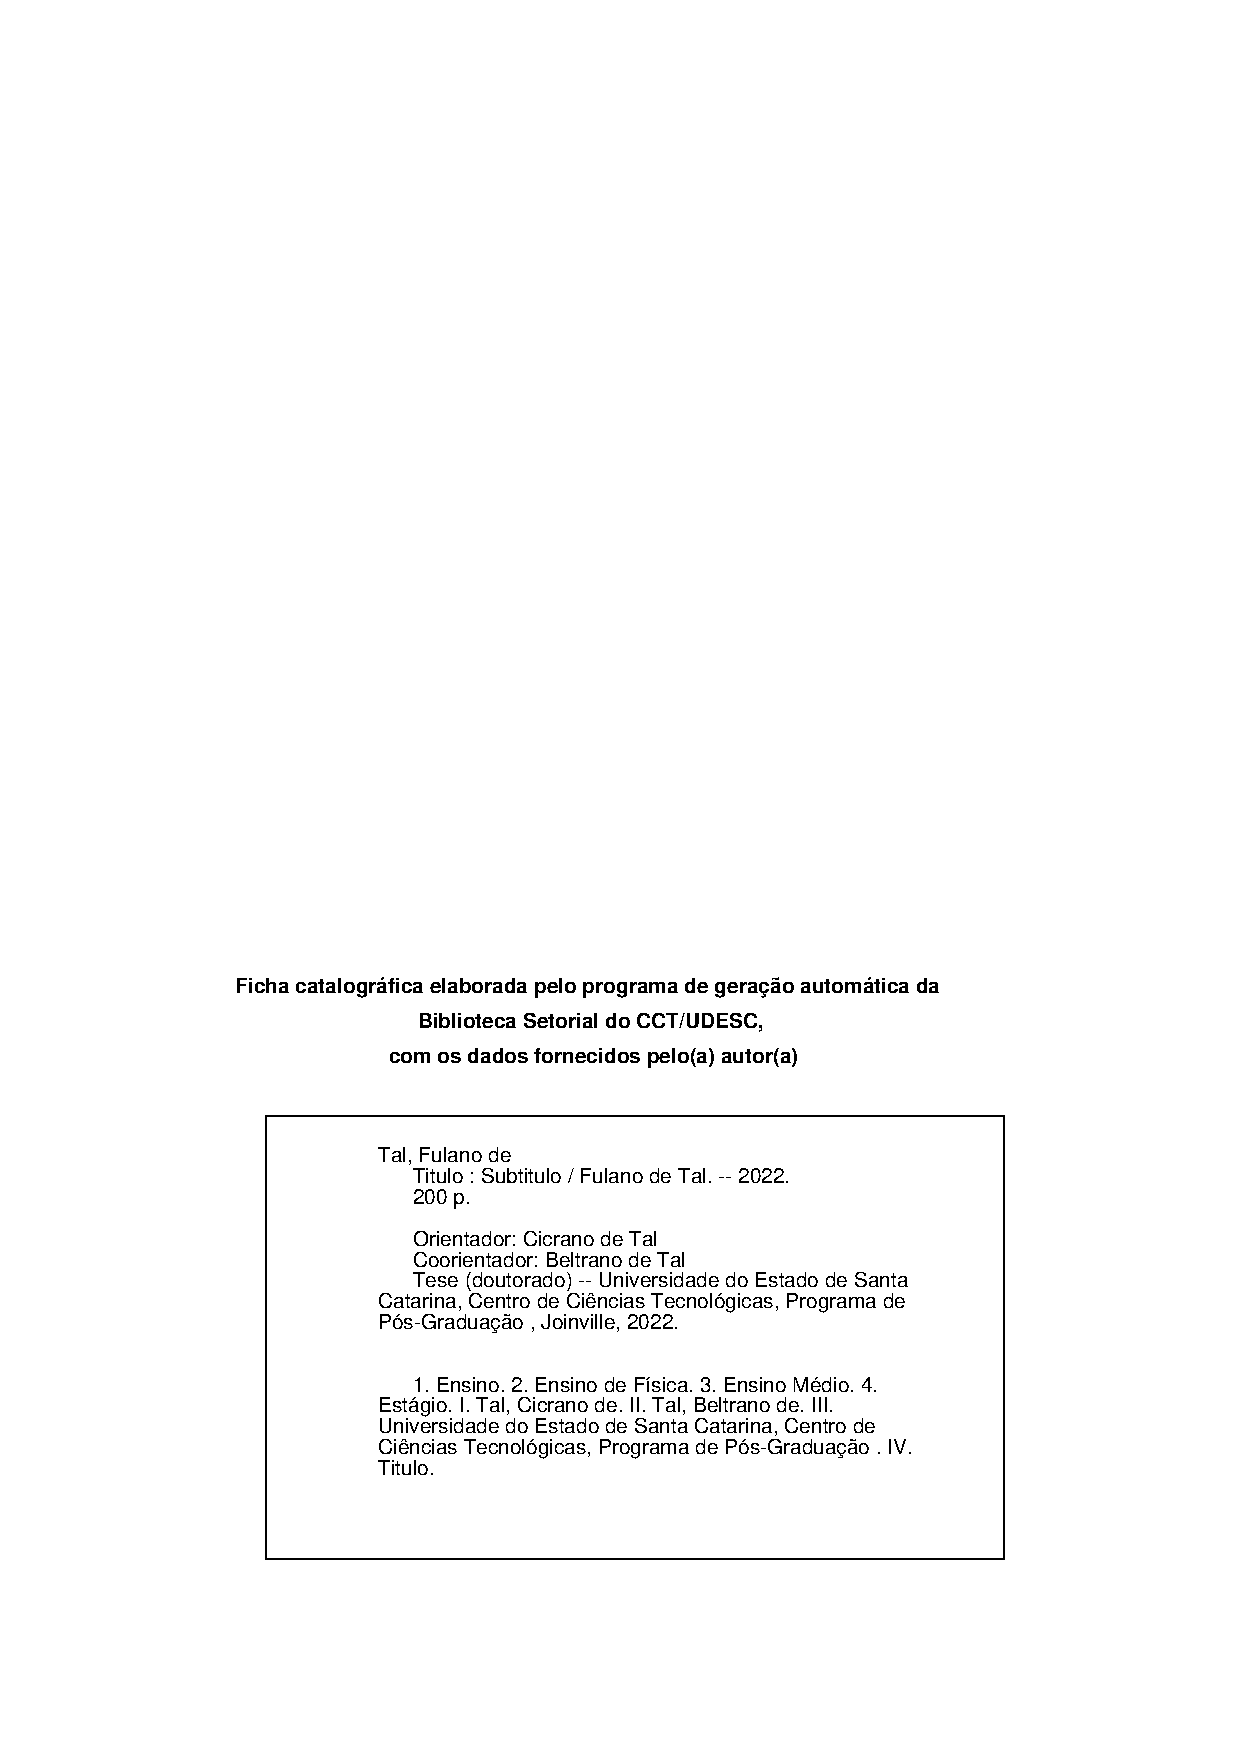
\includepdf[pages=-]{03-elementos/03.1_pre-textual/fichacatalografica.pdf}
%
% \begin{folhadeaprovacao}
%     \textoaprovacao{Este trabalho foi julgado adequado para obtenção do título de Engenheiro de Telecomunicações, pelo Instituto Federal de Educação, Ciência e Tecnologia de Santa Catarina, e aprovado na sua forma final pela comissão avaliadora abaixo indicada.}
%     \begin{center}
%         {\ABNTEXchapterfont\large\MakeUppercase{\imprimirautor}}

%         \vspace*{\fill}\vspace*{\fill}
%         \begin{center}
%             \ABNTEXchapterfont\bfseries\Large\MakeUppercase{\imprimirtitulo}
%         \end{center}
%         \vspace*{\fill}
    
%         \imprimirtextoaprovacao
     
%         \vspace*{1cm}
    
% 	    \imprimirlocal, 6 de maio de 2021:

%     \vspace*{\fill}
%    \end{center}
        


%    \assinatura{\textbf{\imprimirorientador} \\ Orientador\\Instituto Federal de Santa Catarina} 
%    \assinatura{\textbf{Professor Fulano, Dr.} \\ Instituto X }
%    \assinatura{\textbf{Professora Fulana, Dra. } \\ Instituto Y}
%    \assinatura{\textbf{Professor Beltrano, Dr.} \\ Instituto Z}
%    \assinatura{\textbf{Professor} \\ Convidado 4}
      
%     \vspace*{1cm}  
  
% \end{folhadeaprovacao}
%-----------------------------------------------%
%-----------------------------------------------%
% Dedicatória
%-----------------------------------------------%
%
\begin{dedicatoria}
    \vspace*{\fill}    
    \begin{flushright}
        \noindent
        \textit{ Este trabalho é dedicado às crianças adultas que,\\
        quando pequenas, sonharam em se tornar cientistas.}\vspace*{2cm}
    \end{flushright}
\end{dedicatoria}
% ---
% Agradecimentos
%-----------------------------------------------%
%\begin{agradecimentos}
    Os agradecimentos principais são direcionados à Gerald Weber, Miguel Frasson,
    Leslie H. Watter, Bruno Parente Lima, Flávio de Vasconcellos Corrêa, Otavio Real
    Salvador, Renato Machnievscz\footnote{Os nomes dos integrantes do primeiro
    projeto abn\TeX\ foram extraídos de
    \url{http://codigolivre.org.br/projects/abntex/}} e todos aqueles que
    contribuíram para que a produção de trabalhos acadêmicos conforme
    as normas ABNT com \LaTeX\ fosse possível.
    
    Agradecimentos especiais são direcionados ao Centro de Pesquisa em Arquitetura
    da Informação\footnote{\url{http://www.cpai.unb.br/}} da Universidade de
    Brasília (CPAI), ao grupo de usuários
    \emph{latex-br}\footnote{\url{http://groups.google.com/group/latex-br}} e aos
    novos voluntários do grupo
    \emph{\abnTeX}\footnote{\url{http://groups.google.com/group/abntex2} e
    \url{http://www.abntex.net.br/}}~que contribuíram e que ainda
    contribuirão para a evolução do \abnTeX.    
\end{agradecimentos}
% ---
% Epígrafe
%-----------------------------------------------%
%\begin{epigrafe}
    \vspace*{\fill}
	\begin{flushright}
		\textit{Sempre que te perguntarem se podes fazer um trabalho,\\
		respondas que sim e te ponhas em seguida a aprender como se faz.\\
		T. Roosevelt}
	\end{flushright}
\end{epigrafe}
% ---


%-----------------------------------------------%
% RESUMO
%-----------------------------------------------%
\setlength{\absparsep}{18pt} % ajusta o espaçamento dos parágrafos do resumo
\begin{resumo}
    Relatório de estágio desenvolvido na Escola de Educação Básica Giovani Pasqualini Faraco no decorrer do segundo semestre do ano letivo de 2022. Dentre as atividades realizadas e aqui descritas, tem-se: a análise dos documentos oficiais da instituição; observação e análise de aulas da disciplina de Física ministradas pelo professor supervisor além de quinze imersões programadas em atividades de docência, sob orientação técnica do professorao de estágio e custódia do professor supervisor responsável pela disciplina na escola. A cada etapa buscou-se embasar-se na literatura envolvida, e ainda, em consonância com os documentos norteadores da educação básica do país.

\textbf{Palavras-chave}: \firstkey ; \secondkey ; \thirdkey.
\end{resumo}
%-----------------------------------------------%
% ABSTRACT
%-----------------------------------------------%
%\begin{resumo}[Abstract]
    \begin{otherlanguage*}{english}
      This is the english abstract.
   
      \vspace{\onelineskip}
    
      \noindent 
      \textbf{Keywords}: Latex. Abntex. Text editoration.
    \end{otherlanguage*}
\end{resumo}
%-----------------------------------------------%
% ------------------------
% ------------------------
% inserir SUMARIO E LISTAS

% -----------------------------------------------%
% inserir lista de ilustrações, tabelas, listagem 
% de códigos, abreviaturas, símbolos
% -----------------------------------------------%
\pdfbookmark[0]{\listfigurename}{lof}
\listoffigures*
\cleardoublepage
% inserir lista de tabelas
\pdfbookmark[0]{\listtablename}{lot}
\listoftables*
\cleardoublepage

% -----------------------------------------------%
% inserir lista de listings
% -----------------------------------------------%
\pdfbookmark[0]{\lstlistlistingname}{lol}
\begin{KeepFromToc}
\lstlistoflistings
\end{KeepFromToc}
\cleardoublepage
% -----------------------------------------------%

% -----------------------------------------------%
% inserir lista de abreviaturas e siglas
% -----------------------------------------------%
\pdfbookmark[0]{Lista de abreviaturas e siglas}{loa}
%%%%%%%%%%%%%% Como usar o pacote acronym
% \ac{acronimo} -- Na primeira vez que for citado o acronimo, o nome completo irá aparecer
%                  seguido do acronimo entre parênteses. Na proxima vez somente o acronimo
%                  irá aparecer. Se usou a opção footnote no pacote, entao o nome por extenso
%                  irá aparecer aparecer no rodapé
%
% \acf{acronimo} -- Para aparecer com nome completo + acronimo
% \acs{acronimo} -- Para aparecer somente o acronimo
% \acl{acronimo} -- Nome por extenso somente, sem o acronimo
% \acp{acronimo} -- igual o \ac mas deixando no plural com S (ingles)
% \acfp{acronimo}--
% \acsp{acronimo}--
% \aclp{acronimo}--


\chapter*{Lista de abreviaturas e siglas}%
% \addcontentsline{toc}{chapter}{Lista de abreviaturas e siglas}
\markboth{Lista de abreviaturas e siglas}{}

% Para diminuir o espaçamento entre linhas no ambiente de listas acronym
% \let\oldbaselinestretch=\baselinestretch%
% \renewcommand{\baselinestretch}{.2}%
% \large\normalsize%



\begin{acronym}
	\let\oldbaselinestretch=\baselinestretch%
	\renewcommand{\baselinestretch}{.2}%
	\large\normalsize%
	\acro{BNCC}{Base Nacional Comum Curricular}
	\acro{LDB}{Lei de Diretrizes de Bases da Educação Nacional}
	\acro{NEM}{Novo Ensino Médio}
	\acro{PCSC}{Proposta Curricular de Santa Catarina}
	\acro{PNE}{Plano Nacional de Educação}
	\acro{CNE}{Conselho Nacional de Educação}
	\acro{EEB}{Escola de Educação Básica}
	\acro{GPF}{Giovani Pasqualini faraco}
	\acro{EF}{Ensino Fundamental}
	\acro{PPP}{Projeto Político Pedagógico}
	\acro{ATP}{Assistente Técnico Pedagógico}
	\acro{DVD}{\textit{Digital Versatile Disc}}
	\acro{EI}{Ensino por Investigação}
	\acro{NI/D}{Não-Interativo/Dialógico}
	\acro{I/D}{Interativo-Dialógico}
	\acro{HC}{História da Ciência}
	\acro{TIC}{Tecnologia da Informação e Comunicação}
	\acro{ENEM}{Exame Nacional do Ensino Médio}
	\acro{I/DA}{Interativo/Dialógico de Autoridade}
\end{acronym}

\cleardoublepage
% -----------------------------------------------%

% -----------------------------------------------%
% inserir lista de símbolos
% -----------------------------------------------%
\begin{simbolos}
  \item[$ \Gamma $] Letra grega Gama
  \item[$ \Lambda $] Lambda
  \item[$ \zeta $] Letra grega minúscula zeta
  \item[$ \in $] Pertence
\end{simbolos}
% -----------------------------------------------%

% -----------------------------------------------%
% inserir o sumario
% -----------------------------------------------%
\pdfbookmark[0]{\contentsname}{toc}
\tableofcontents*
\cleardoublepage
% -----------------------------------------------%
% ------------------------

%-----------------------------------------------%
% ELEMENTOS TEXTUAIS
%-----------------------------------------------%
\textual
% Se quiser que apareça o título dos capítulos
% no cabeçalho, então comente a linha abaixo
%\pagestyle{cabecalholimpo}
%-----------------------------------------------%
% Inclusão dos capítulos que estão em outros arquivos .tex
%-----------------------------------------------%
\chapter{Introdução}
\label{c_introducao}

A introdução abre o trabalho propriamente dito. Tem a finalidade de apresentar os motivos que levaram o autor a realizar a pesquisa, o problema abordado, os objetivos e a justificativa. O objetivo principal da introdução é situar o leitor no contexto da pesquisa. O leitor deverá perceber claramente o que foi analisado, como e por que, as limitações encontradas, o alcance da investigação e suas bases teóricas gerais. Ela tem, acima de tudo, um caráter didático de apresentar o que foi investigado, levando-se em conta o leitor a que se destina e a finalidade do trabalho.

Assim, na introdução contextualize o tema, delimite o assunto, apresente um rápido histórico do problema e das soluções porventura já apresentadas, com breve revisão crítica das investigações anteriores; faça referência às fontes de material, aos métodos seguidos, às teorias ou aos conceitos que embasam o desenvolvimento e a argumentação, às eventuais faltas de informação, ao instrumental utilizado. A introdução deverá conter, ainda:

\begin{enumerate}
   \item Justificativa;
   \item Definição do problema;
   \item Objetivo geral e objetivos específicos.
\end{enumerate}


% ---
\section{Compilar o documento \LaTeX}
% ---

É uma boa prática dividir o seu documento em diversos arquivos, e não apenas escrever tudo em um único. Esse recurso foi utilizado neste documento. Para incluir diferentes arquivos em um arquivo principal, de modo que cada arquivo incluído fique em uma página diferente, utilize o comando:

\begin{verbatim}
   \include{documento-a-ser-incluido}      % sem a extensão .tex
\end{verbatim}

Para incluir documentos sem quebra de páginas, utilize:

\begin{verbatim}
   \input{documento-a-ser-incluido}      % sem a extensão .tex
\end{verbatim}

Geralmente os editores \LaTeX, como o
TeXlipse\footnote{\url{http://texlipse.sourceforge.net/}}, o
Texmaker\footnote{\url{http://www.xm1math.net/texmaker/}}, entre outros,
compilam os documentos automaticamente, de modo que você não precisa se
preocupar com isso.

No entanto, você pode compilar os documentos \LaTeX usando os seguintes
comandos, que devem ser digitados no \emph{Prompt de Comandos} do Windows ou no
\emph{Terminal} do Mac ou do Linux:

\begin{verbatim}
   pdflatex ARQUIVO_PRINCIPAL.tex
   bibtex ARQUIVO_PRINCIPAL.aux
   makeindex ARQUIVO_PRINCIPAL.idx 
   makeindex ARQUIVO_PRINCIPAL.nlo
   pdflatex ARQUIVO_PRINCIPAL.tex
   pdflatex ARQUIVO_PRINCIPAL.tex
\end{verbatim}

% ---
\section{Referências bibliográficas}
% ---

A formatação das referências bibliográficas conforme as regras da ABNT são um
dos principais objetivos do \abnTeX. Consulte os manuais
%\citeonline{abntex2cite} e \citeonline{abntex2cite-alf} para obter informações
sobre como utilizar as referências bibliográficas.

%-
\subsection{Acentuação de referências bibliográficas}
%-

Normalmente não há problemas em usar caracteres acentuados em arquivos
bibliográficos (\texttt{*.bib}). Porém, como as regras da ABNT fazem uso quase
abusivo da conversão para letras maiúsculas, é preciso observar o modo como se
escreve os nomes dos autores. Na ~\autoref{tabela-acentos} você encontra alguns
exemplos das conversões mais importantes. Preste atenção especial para `ç' e `í'
que devem estar envoltos em chaves. A regra geral é sempre usar a acentuação
neste modo quando houver conversão para letras maiúsculas.

\begin{table}[htbp]
\caption{Tabela de conversão de acentuação.}
\label{tabela-acentos}

\begin{center}
\begin{tabular}{ll}\toprule
acento & \textsf{bibtex}\\\midrule
à á ã & \verb+\`a+ \verb+\'a+ \verb+\~a+\\
í & \verb+{\'\i}+\\
ç & \verb+{\c c}+\\
\bottomrule
\end{tabular}
\end{center}
\end{table}




\section{Motivação}
\label{ci_s_motivacao}

A motivação deste documento foi a necessidade da elaboração de modelo para a concepção de monografias para o IFSC. 

\section{Organização do texto}
\label{ci_s_organizacao}

O texto está organizado da seguinte forma: No \autoref{c_cap2} é apresentado um pouco mais de como fazer um outro capítulo, apresentando ainda formas para inserir figuras. No \autoref{c_cap3} é apresentado uma forma para adicionar uma tabela. Por fim, no \autoref{c_conclusoes} são apresentadas as conclusões sobre este trabalho.
% ----------------------------------------------------------------------- %
% Arquivo: cap2.tex
% ----------------------------------------------------------------------- %

\chapter{Alguns conceitos}
\label{c_cap2}

É a parte principal do texto. Apresenta o assunto, fundamentação teórica, metodologia (materiais e métodos), os resultados e as respectivas discussões traçando relações com os trabalhos analisados na revisão de literatura.

\section{Revisão de literatura}\label{s_c2_revisao}

É uma análise comentada sobre o que já foi publicado sobre o assunto da pesquisa, buscando mostrar os pontos de vista convergentes e divergentes entre os autores. Traça-se um quadro teórico e elabora-se a estruturação conceitual que subsidiará o desenvolvimento da pesquisa. A revisão de literatura permitirá um mapeamento de quem já escreveu e o que já foi escrito sobre o assunto ou o problema de pesquisa.







\section{A inclusão de figuras}
\label{s_c2_figuras}

As figuras são bastante úteis para ajudar expressar o funcionamento, modelo, etc. de alguma parte de seu trabalho. No Linux existem diversas aplicações para a criação de figuras, sendo o Xfig\footnote{\url{http://www.xfig.org}} uma ótima opção para a criação de figuras com alta qualidade, apesar de sua interface não ser muito amigável. Muitos utilizam outras aplicações com interfaces mais amigáveis e que ainda assim geram figuras com uma qualidade razoável como o \textit{Inkscape}, \textit{DIA}, \textit{OpenOffice Draw}, \textit{Kivio}, etc.

A inclusão de figuras no texto necessita que algumas regras sejam atendidas. São essas:

\begin{itemize}
	\item As figuras deverão ser de alta qualidade;
	\begin{itemize}
		\item Evite colocar fotos e outras figuras complexas;
		\item Opte por figuras simples e que realmente expressem algo, mesmo quando impressas em preto e branco;
	\end{itemize}
	\item Em \LaTeX~as figuras deverão estar nos formatos: \texttt{PDF}, \texttt{JPG} ou \texttt{PNG};
	\item Toda figura deverá possuir uma legenda;
	\item Toda figura deverá ser referenciada em alguma parte do texto.
\end{itemize}

A \autoref{f_c2_disco} foi inserida no texto para mostrar como fazer tal inserção em \LaTeX. Vale lembrar que toda figura inserida deverá ser, em algum momento, referenciada no texto. 

\begin{figure}[!htpb]
	\centering
	\caption{Disquete}\label{f_c2_disco}
	%\includegraphics[width=5cm]{03.2.1_fig/disco}
    \includegraphics[width=5cm]{03-elementos/03.2_textual/03.2.1_fig/disco.pdf}
\end{figure}

O objetivo deste documento é de mostrar como preparar uma monografia para o curso de Engenharia de Telecomunicações. No ~\autoref{c_cap3} é apresentado uma forma para fazer citações de outros trabalhos. O capítulo ainda apresenta uma forma para incluir tabelas no documento. O ~\autoref{c_conclusoes} apresenta as conclusões deste trabalho além de apresentar os trabalhos futuros.

\subsection{Mascotes}
\label{s_c2_mascotes}

Essa é uma subseção da \autoref{s_c2_figuras} do \autoref{c_cap2}. 

\begin{figure}[ht]
	\centering
	\caption{O mascote do~\LaTeX~em diferentes poses}\label{f_c2_mascotes}
	\subcaptionbox{O mascote estudando\label{f_c2_masco1}}
		{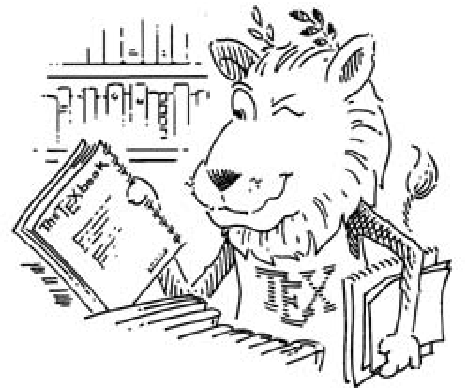
\includegraphics[width=.4\textwidth]{03-elementos/03.2_textual/03.2.1_fig/lion.pdf}}
	\subcaptionbox{O mascote ensinando\label{f_c2_masco2}}
		{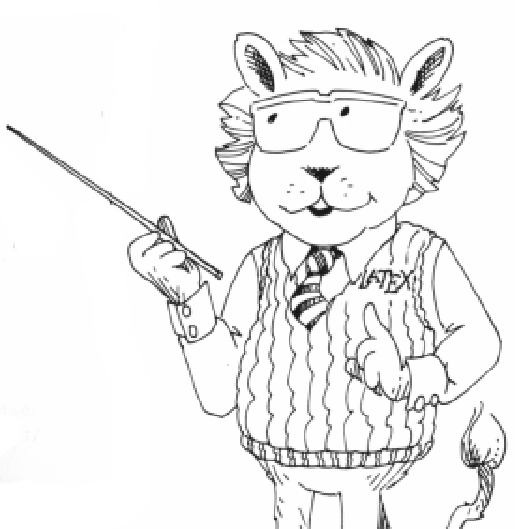
\includegraphics[width=.4\textwidth]{03-elementos/03.2_textual/03.2.1_fig/latex_lion.pdf}}
\end{figure}


A \autoref{f_c2_mascotes} ilustra uma forma de incluir duas figuras, lado a lado, usando o pacote \texttt{subcaption}. A \autoref{f_c2_masco1} ilustra o mascote do \LaTeX~estudando. Já na \autoref{f_c2_masco2} o mascote aparece apresentando algum assunto. 


\section{Como apresentar equações}
\label{s_c2_equacoes}

O \LaTeX é um pacote feito para a preparação de textos impressos de alta qualidade, especialmente
para textos matemáticos. Ele foi desenvolvido por Leslie Lamport a partir do programa
\TeX~criado por Donald Knuth.

Fórmulas matemáticas são produzidas digitando no arquivo fonte texto descrevendo-as. Isto
significa que o \LaTeX~deve ser informado que o texto que vem a seguir é uma fórmula e também
quando ela termina e o texto normal recomeça. As fórmulas podem ocorrer em uma linha de
texto como $ax^2 + bx + c = 0$, ou destacada do texto principal como na \autoref{e_c2_eq1}.

\begin{equation}
 x=\frac{-b\pm\sqrt{b^2-4ac}}{2a}
\label{e_c2_eq1}
\end{equation}

\section{Incluindo trechos de códigos}

Em alguns casos é desejado incluir trechos de códigos no documento. O \LaTeX oferece inúmeras maneiras para isto e o pacote \textbf{listings} é conhecido por apresentar um dos melhores resultados. A \autoref{l_olamundo} apresenta o código em \textit{shell script} para o complexo problema do ``Olá mundo!''. A \autoref{l_matlab} apresenta um trecho de código em MatLab.

%parâmetros: linguagem (shell, java, matlab, python, c, php), label, caption, arquivo

\includecode[shell]{l_olamundo}{Olá mundo em shell script}{03-elementos/03.2_textual/03.2.0_codes/ola.sh}

\includecode[matlab]{l_matlab}{Um pequeno código em MatLab}{03-elementos/03.2_textual/03.2.0_codes/matlab.m}

% ---
\section{Divisões do documento: seção}\label{sec-divisoes}
% ---

Esta seção testa o uso de divisões de documentos. Esta é a
\autoref{sec-divisoes}. Veja a \autoref{sec-divisoes-subsection}.

\subsection{Divisões do documento: subseção}\label{sec-divisoes-subsection}

Isto é uma subseção. Veja a \autoref{sec-divisoes-subsubsection}, que é uma
\texttt{subsubsection} do \LaTeX, mas é impressa chamada de ``subseção'' porque
no Português não temos a palavra ``subsubseção''.

\subsubsection{Divisões do documento: subsubseção}
\label{sec-divisoes-subsubsection}

Isto é uma subsubseção.

\subsubsection{Divisões do documento: subsubseção}

Isto é outra subsubseção.

\subsection{Divisões do documento: subseção}\label{sec-exemplo-subsec}

Isto é uma subseção.

\subsubsection{Divisões do documento: subsubseção}

Isto é mais uma subsubseção da \autoref{sec-exemplo-subsec}.


\subsubsubsection{Esta é uma subseção de quinto
nível}\label{sec-exemplo-subsubsubsection}

Esta é uma seção de quinto nível. Ela é produzida com o seguinte comando:

\begin{verbatim}
\subsubsubsection{Esta é uma subseção de quinto nível}
\label{sec-exemplo-subsubsubsection}
\end{verbatim}

\subsubsubsection{Esta é outra subseção de quinto nível}\label{sec-exemplo-subsubsubsection-outro}

Esta é outra seção de quinto nível.


\paragraph{Este é um parágrafo numerado}\label{sec-exemplo-paragrafo}

Este é um exemplo de parágrafo nomeado. Ele é produzida com o comando de
parágrafo:

\begin{verbatim}
\paragraph{Este é um parágrafo nomeado}
\label{sec-exemplo-paragrafo}
\end{verbatim}

A numeração entre parágrafos numeradaos e subsubsubseções são contínuas.

\paragraph{Esta é outro parágrafo numerado}\label{sec-exemplo-paragrafo-outro}

Esta é outro parágrafo nomeado.

% ---
\section{Este é um exemplo de nome de seção longo. Ele deve estar
alinhado à esquerda e a segunda e demais linhas devem iniciar logo abaixo da
primeira palavra da primeira linha}
% ---

Isso atende à norma \citeonline[seções de 5.2.2 a 5.2.4]{NBR14724:2011} 
 e \citeonline[seções de 3.1 a 3.8]{NBR6024:2012}.


\section{Usando siglas e abreviaturas}

Algumas vezes nos deparamos com textos cheios de siglas. O \LaTeX provê ferramentas para gerar glossário, lista de acrônimos, etc. Neste parágrafo é feito uso de comandos definidos no pacote \textit{acronym} e a listagem de acrônimos fica dentro do arquivo \texttt{abreviaturas.tex}.

O protocolo \ac{TLS} deve ser empregado sempre que se deseja garantir a integridade e a confidencialidade das mensagens trocadas pela rede. O \ac{TLS} é hoje utilizado por diversas aplicações. Como faz tempo que eu não falo do \acf{TLS} eu chamo o nome completo mais a sigla, ajudando o meu leitor a lembrar da sigla \ac{TLS}. Existe a \ac{AC} que é bem importante. Este documento segue as normas da \ac{ABNT} e para isso faz uso do pacote \ac{abnTeX}.
\chapter{Apoio à Docência}
\label{cap: apoioDocencia}
Neste capítulo, apresentaremos os principais recursos físicos e estruturais da \ac{GPF}, disponíveis aos docentes para melhor desempenharem suas atividades.

\section{Sala dos Professores}
\setlength\intextsep{0pt}
\begin{wrapfigure}[9]{r}{0.5\textwidth}
    \centering
    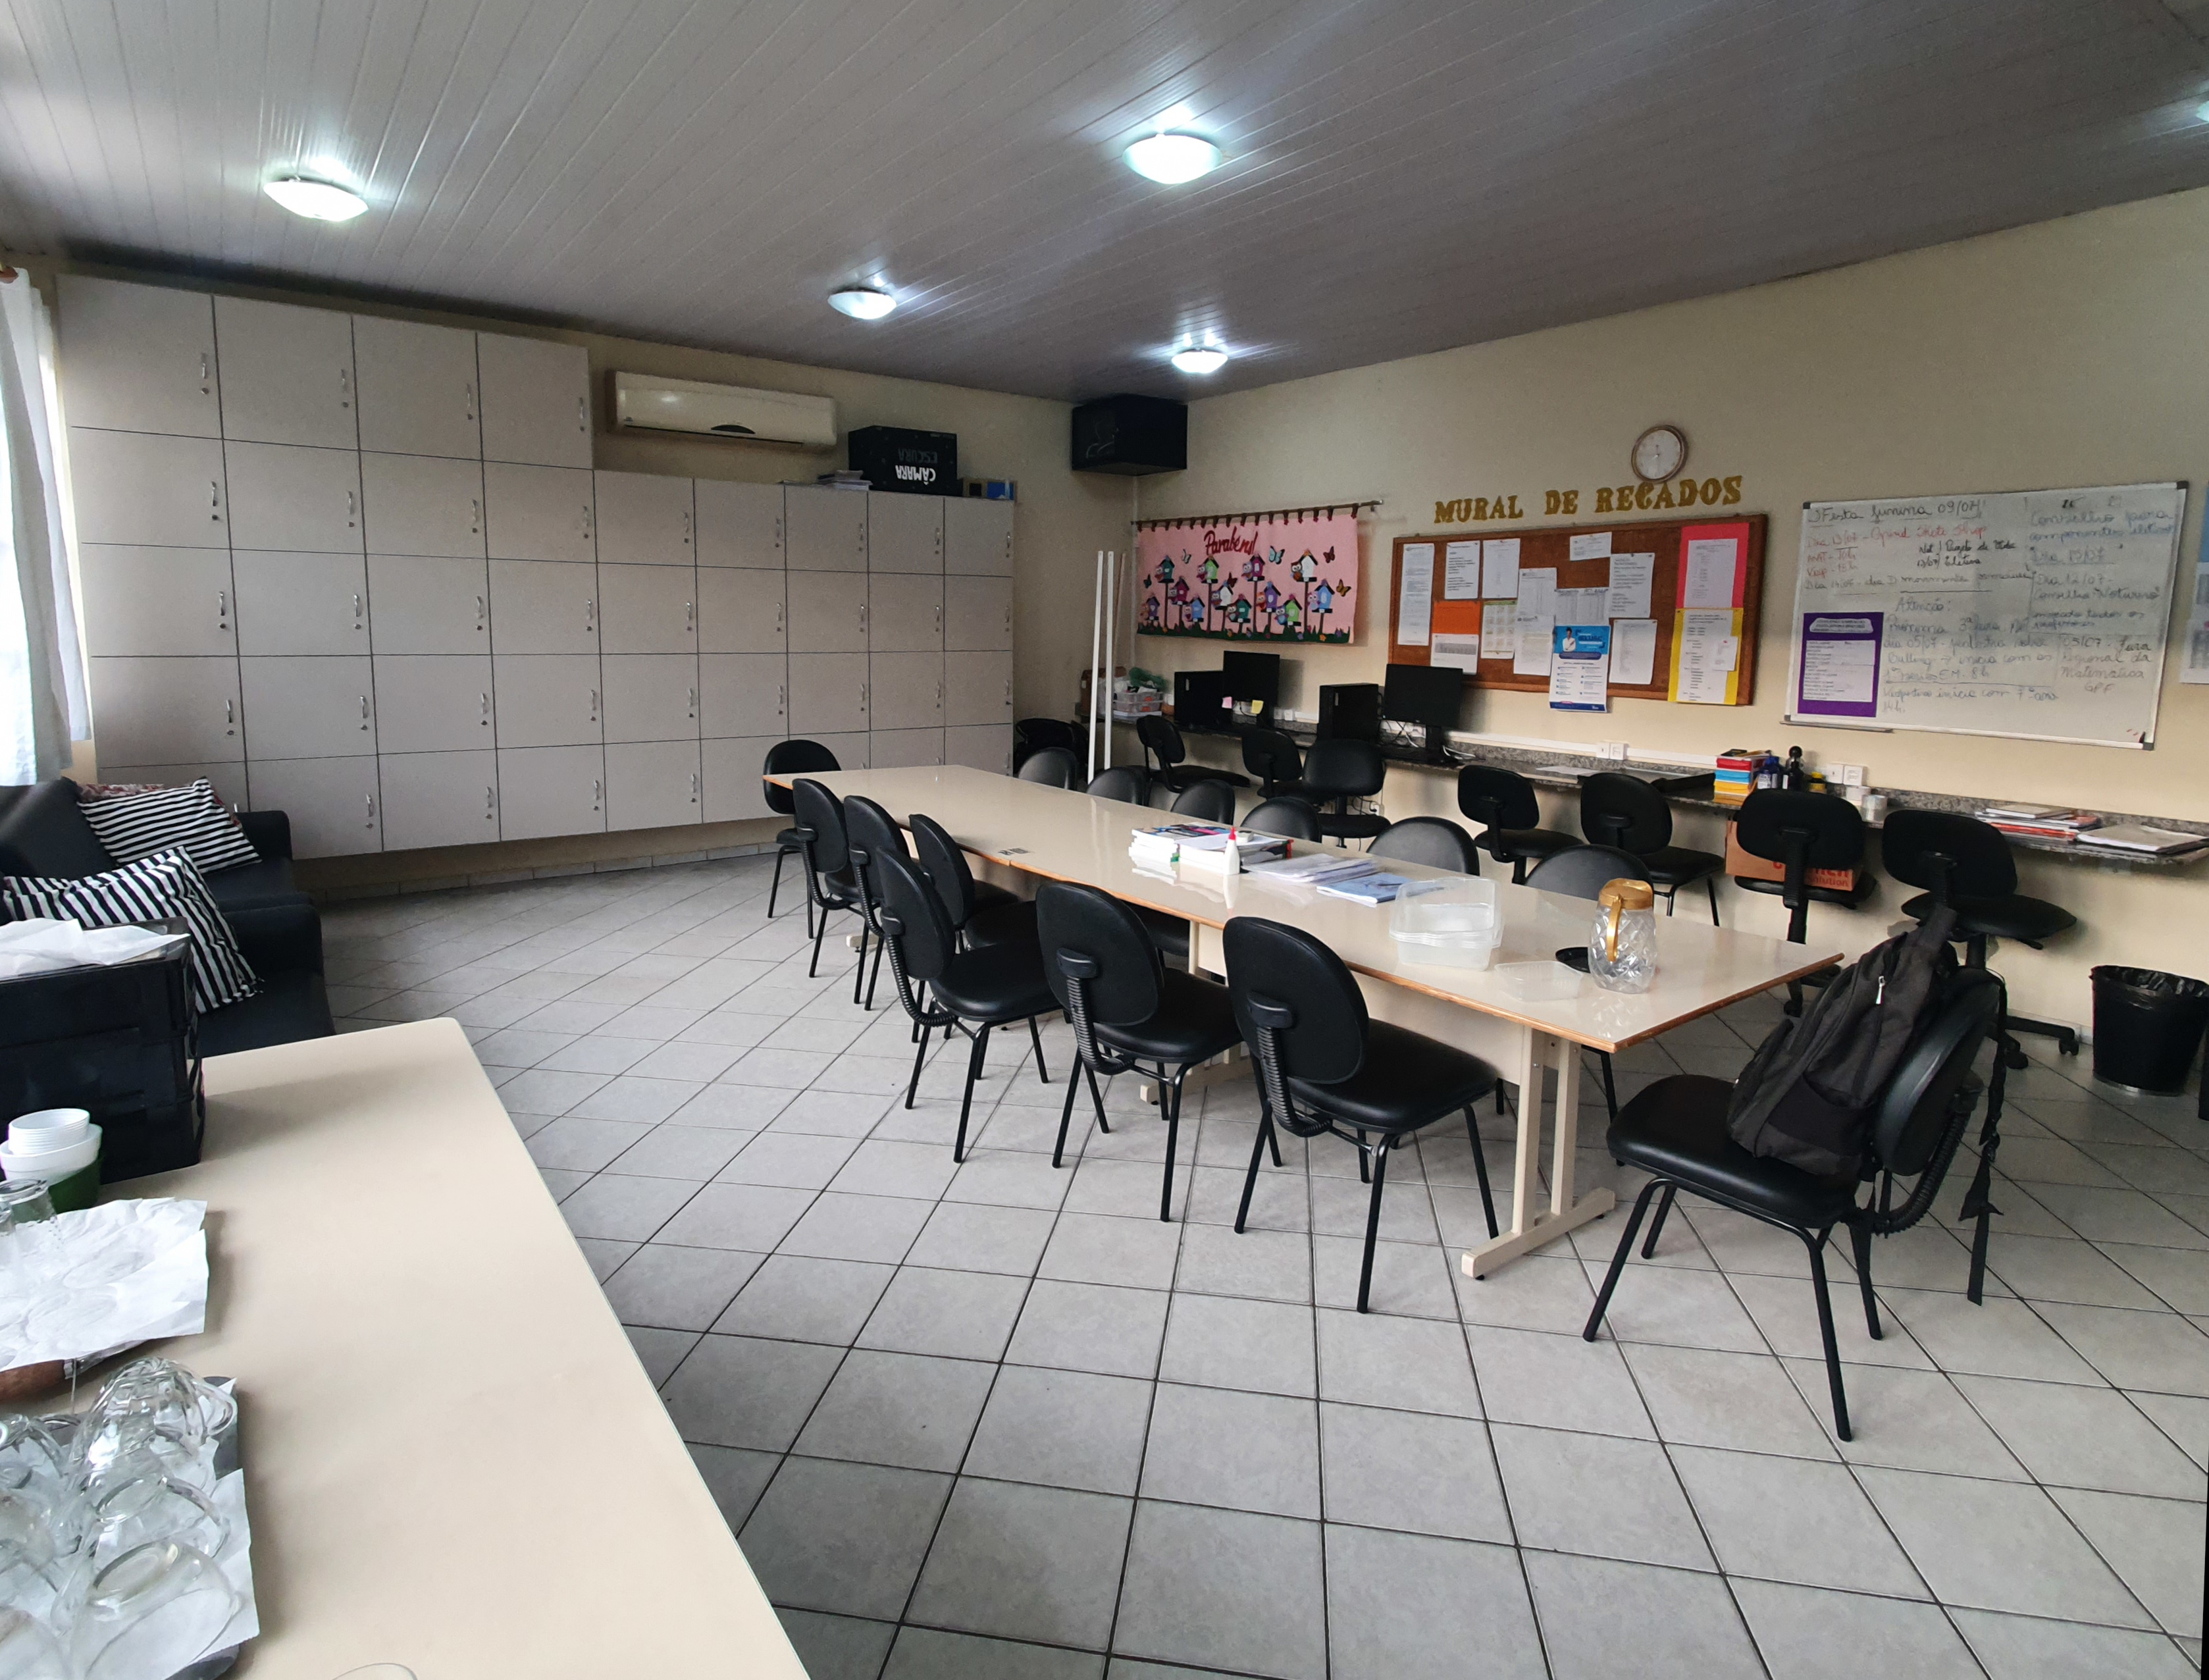
\includegraphics[width=.45\textwidth]{03-elementos/03.2_textual/03.2.1_fig/sala-de-profs01.jpg}
    
    \label{fig:salaDosProfs}
    \caption{Sala dos Professores}    
\end{wrapfigure}
Bem espaçosa a Sala dos Professores possui: geladeira, microondas, ar-condicionado e um purificador de água. É equipada com dois desktops conectados à internet. Cada professor tem um espaço nos armários, e é nele que fica guardado o \emph{Data-Show} para uso em aulas diferenciadas.

\section{Laboratório}
As aulas experimentais podem ser conduzidas no Laboratório, preparado para atender as disciplinas de Física, Química e Biologia. Comporta cerca de 40 alunos, e é composto por duas grandes bancadas e alguns armários. Infelizmente no momento em que este relatório foi escrito, encontrava-se interditado devido à alocação dos materiais para montar a festa junina. Dessa forma, a entrada ao laboratório estava restrita apenas para a equipe gestora.

\section{Laboratório de informática}
\setlength\intextsep{0pt}
\begin{wrapfigure}[9]{l}{0.5\textwidth}
    \centering
    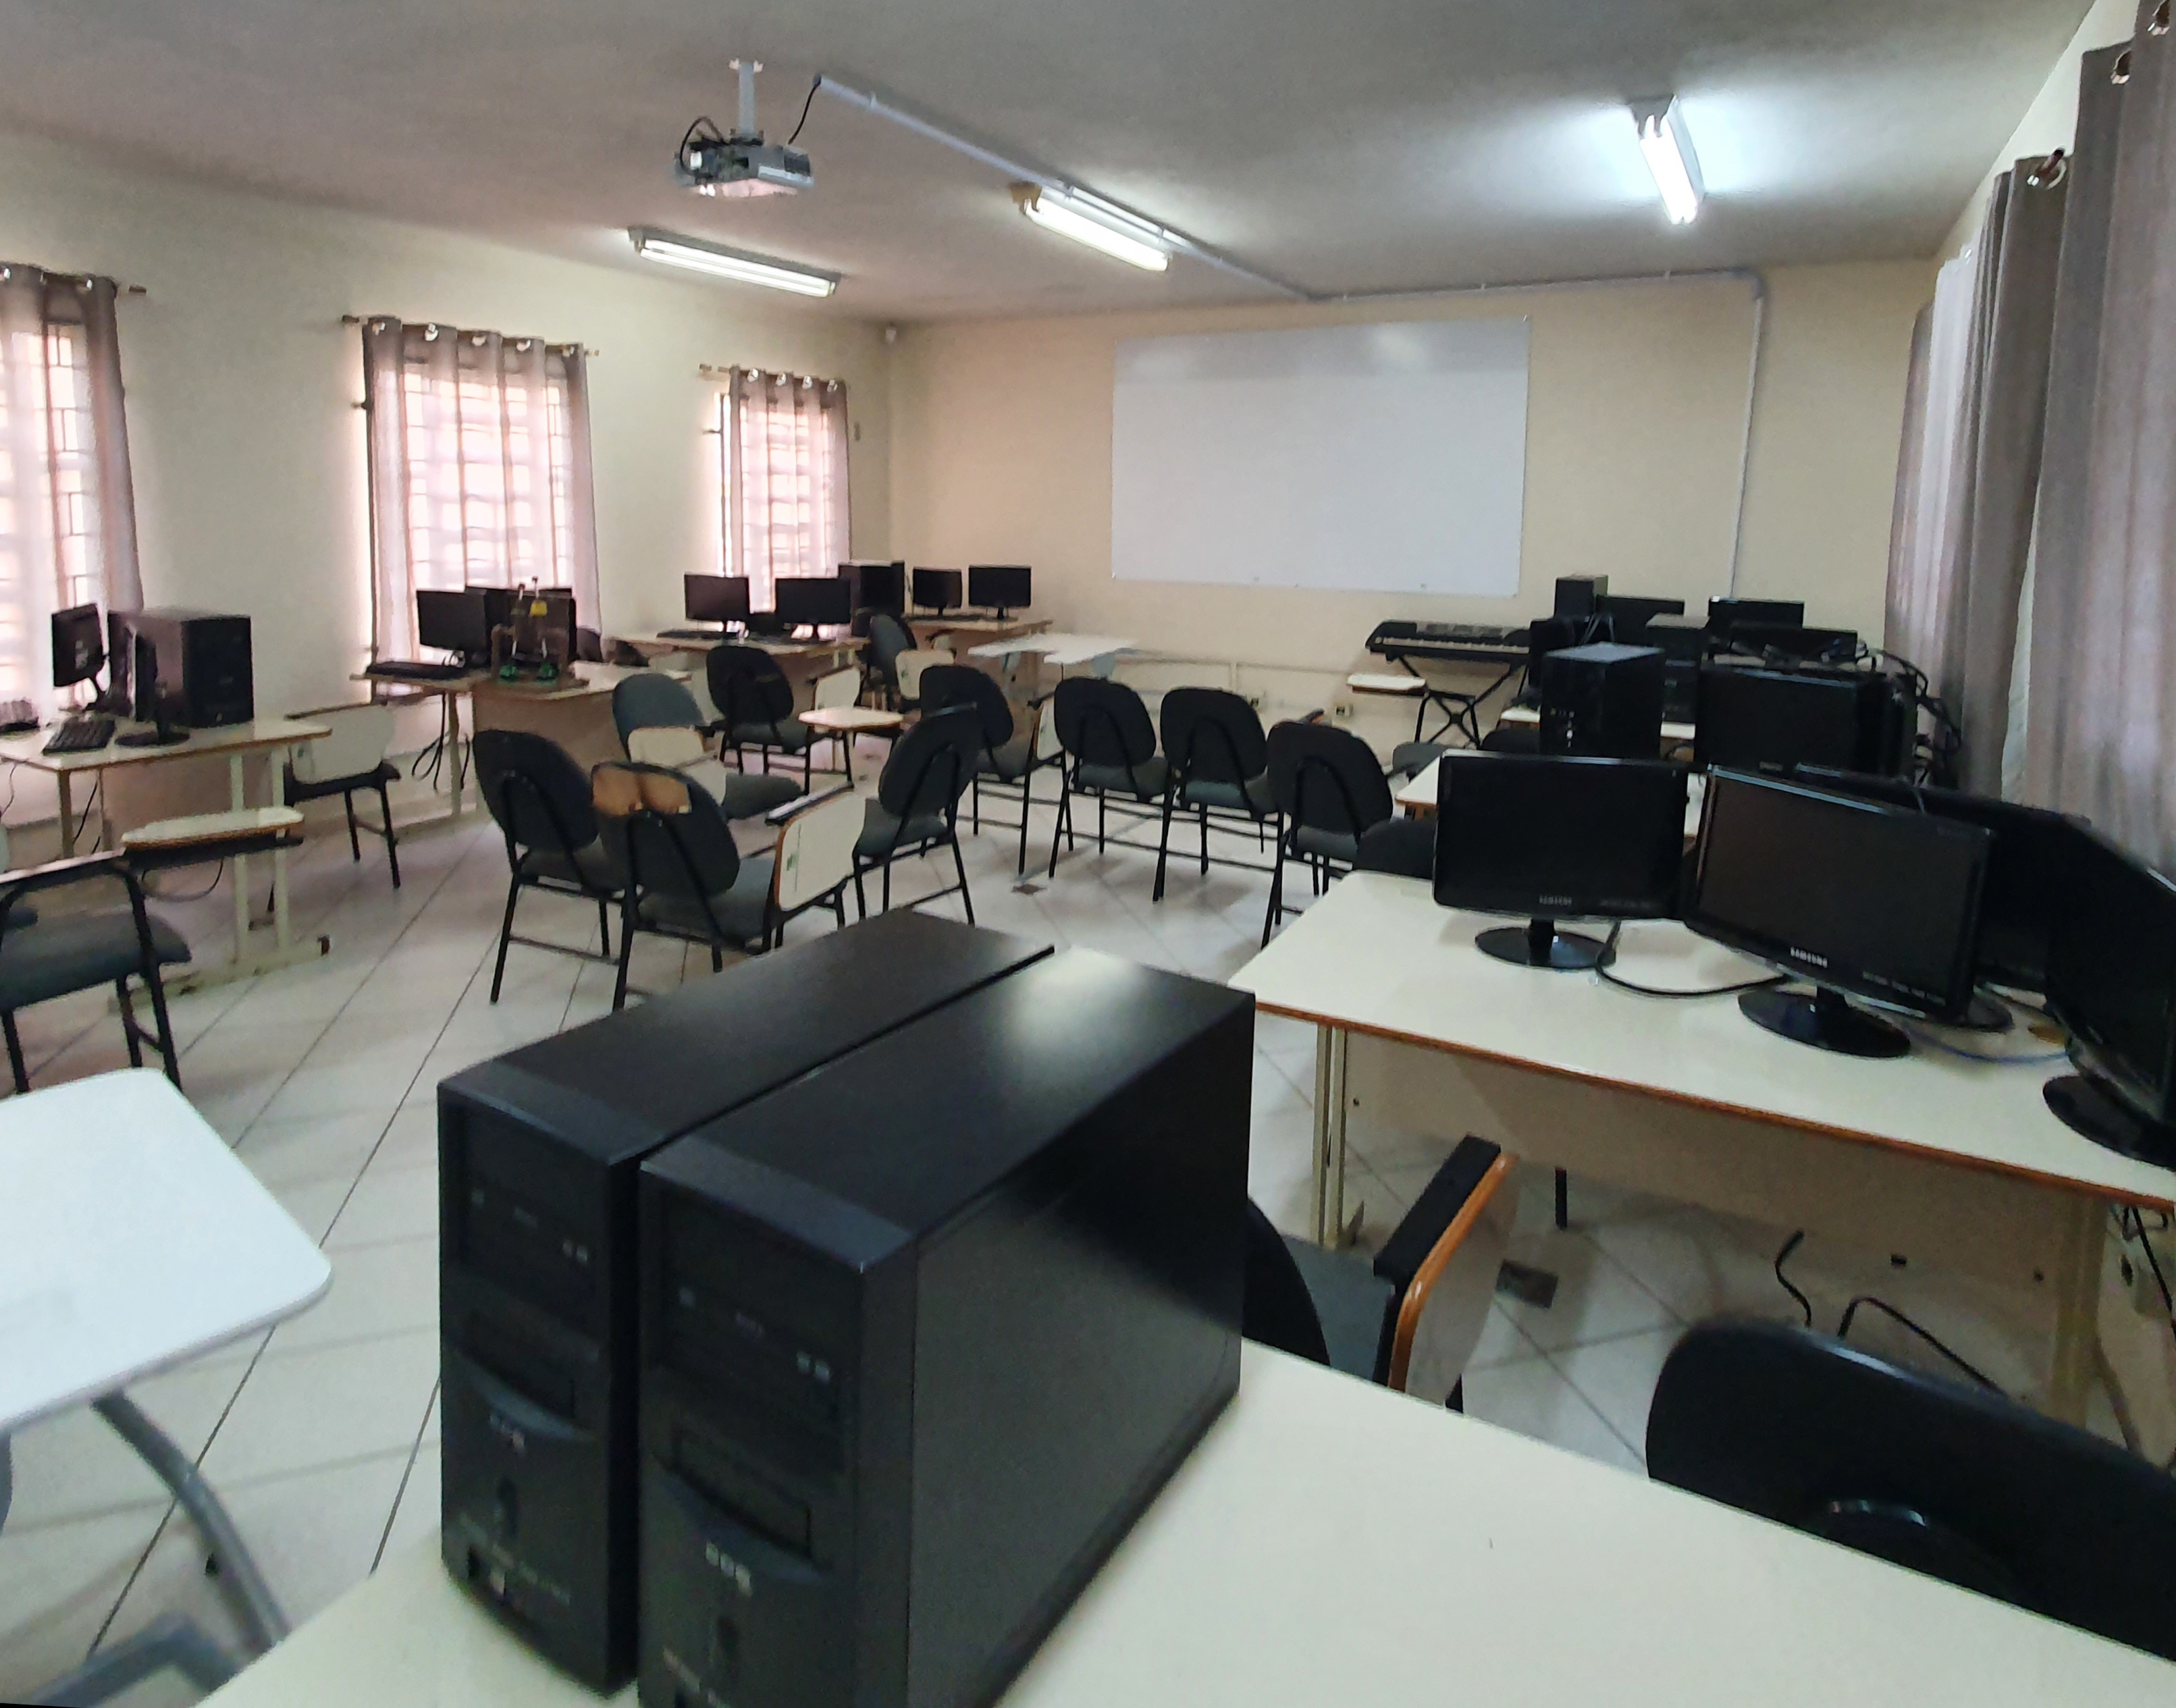
\includegraphics[width=.45\textwidth]{03-elementos/03.2_textual/03.2.1_fig/sala-de-informatica02.jpg} 
    \caption{Laboratório de informática}
    \label{fig:salaDeInformatica}  
\end{wrapfigure}
O Laboratório de Informática é composto por 9 desktops e 19 monitores com acesso à internet, tem capacidade para atender até 19 alunos em virtude da quantidade de dispositivos. Possui ainda uma Lousa Melamínica ($350\times 120$)\cm\; e retroprojetor.

\section{Salas de aula}
As Salas de Aulas são planejadas para comportar em média 30 alunos. Boa parte das salas possuem ar-condicionados, armários e são devidamente equipadas com Lousa Melamínica ($400\times 120$)\cm.

\section{Auditório}
\setlength\intextsep{0pt}
\begin{wrapfigure}[9]{r}{0.4\linewidth}
    \centering
    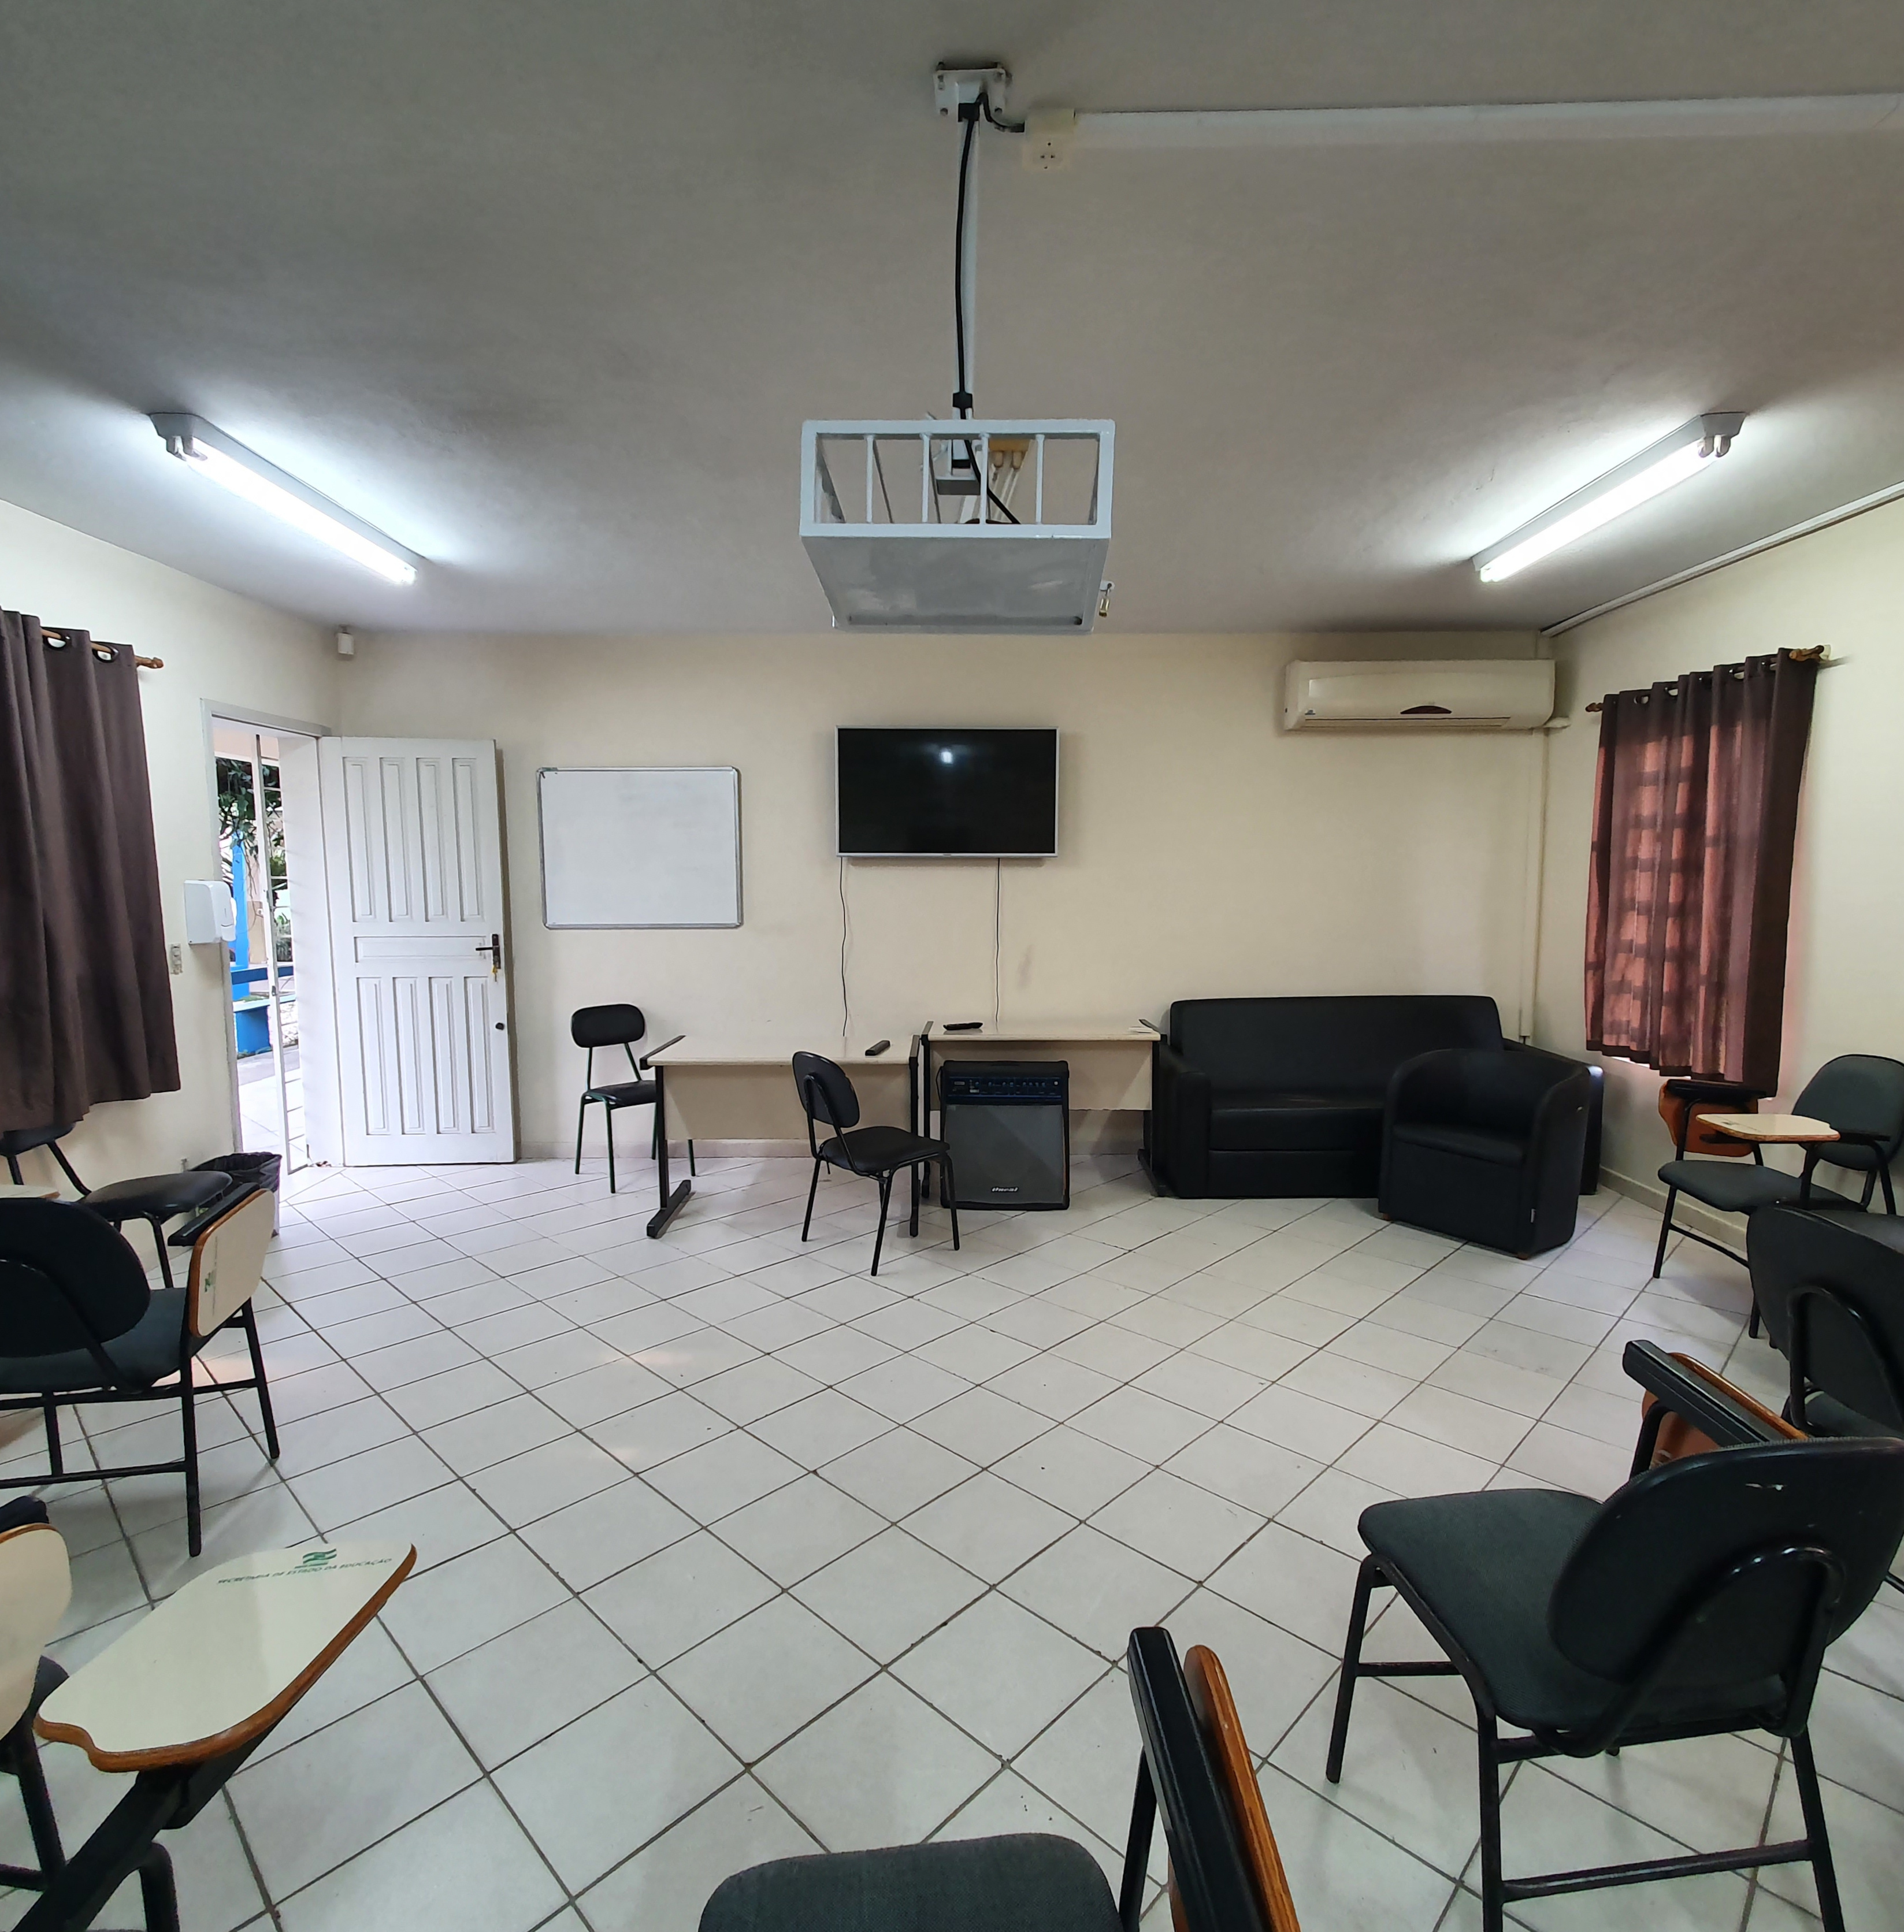
\includegraphics[width=.35\textwidth]{03-elementos/03.2_textual/03.2.1_fig/auditorio01.jpg} 
    \caption{Auditório}
    \label{fig:auditorio}    
\end{wrapfigure}
O auditório tem capacidade para comportar um total 40 pessoas, é equipado com: um televisor de led $40\inch$, caixa de som amplificada multiuso Oneal-OCM modelo 550 de $80\Watt$ de potência rms, um retroprojetor e ar-condicionado.

\section{Biblioteca}
No acervo da Biblioteca encontram-se: livros didáticos de todas as disciplinas, livros de literatura nacional e internacional, almanaques, \acp{DVD} educativos, revistas de assuntos dos mais variádos e jornais. Possui também uma televisão de $32\inch$ a tubo conectada à uma leitora de \ac{DVD}, mesas e cadeiras o suficiente para comportar uma pequena turma de 10 pessoas.
\vfill
\begin{figure}[!ht]
    \begin{center}
        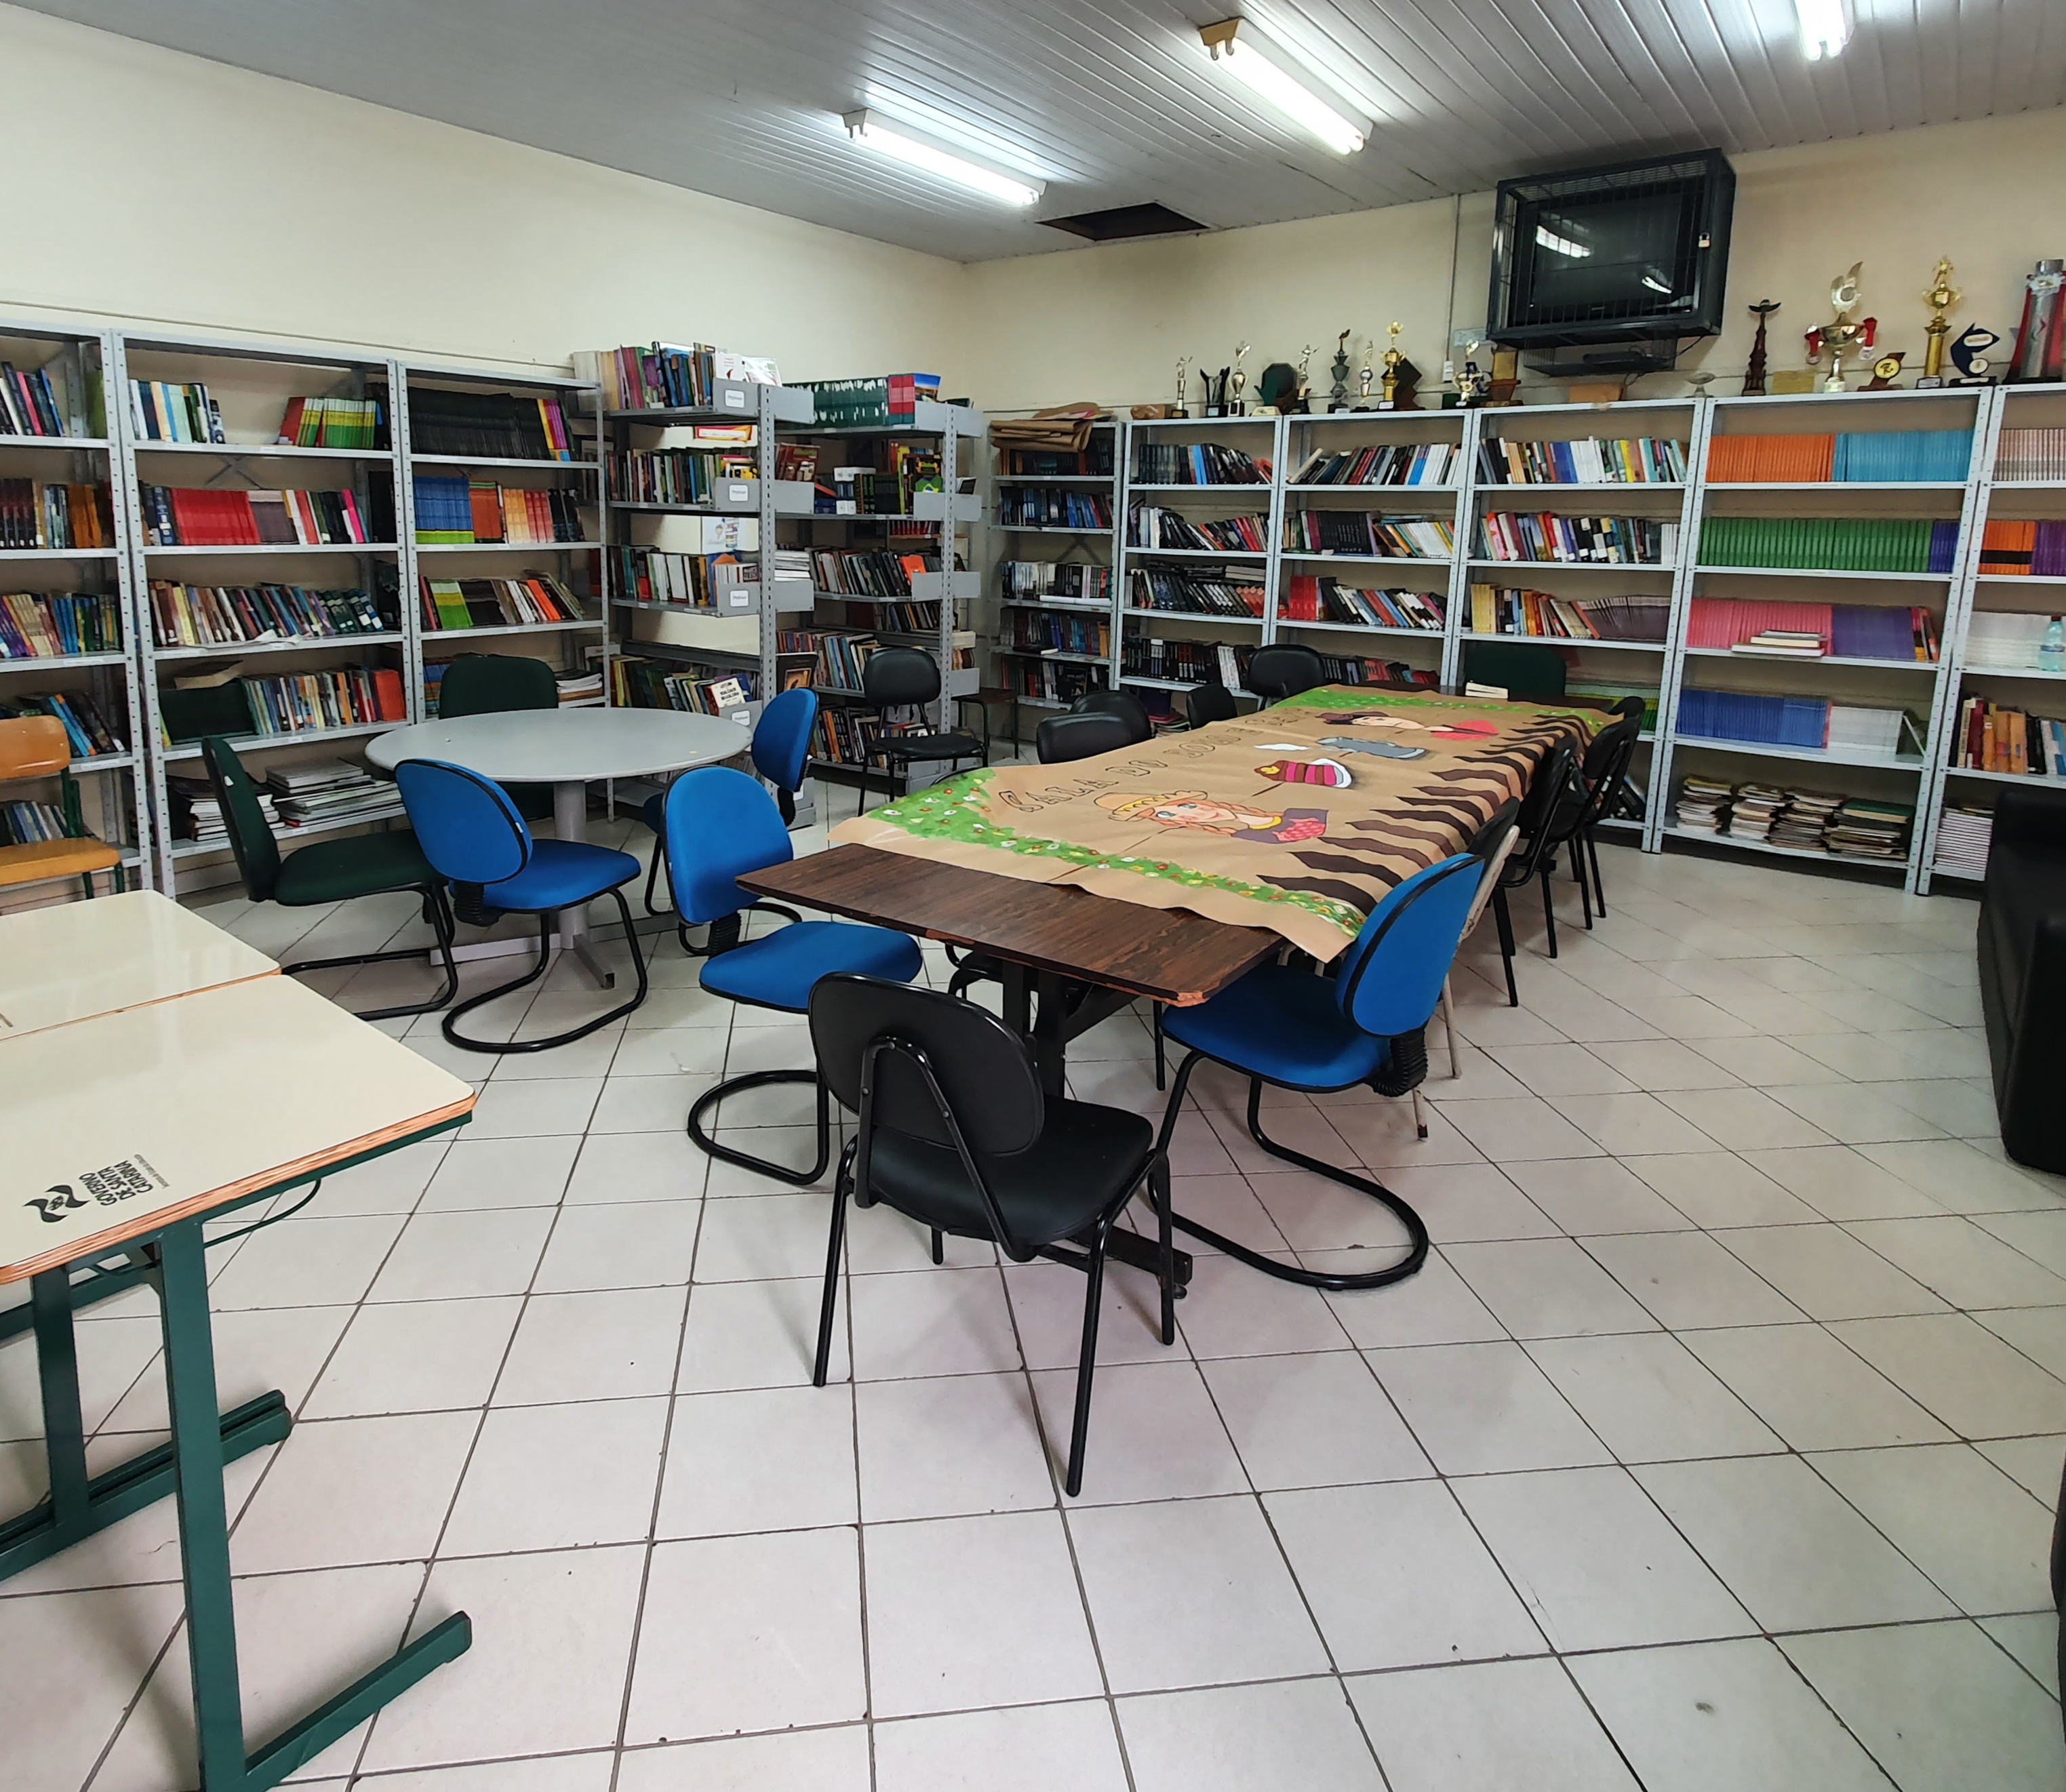
\includegraphics[width=.7\textwidth]{03-elementos/03.2_textual/03.2.1_fig/biblioteca01.jpg}       
        \label{fig:biblioteca}    
        \caption{Biblioteca}
    \end{center}    
\end{figure}




% ----------------------------------------------------------------------- %
% Arquivo: conclusoes.tex
% ----------------------------------------------------------------------- %

\chapter{Conclusões}
\label{c_conclusoes}

Este trabalho procurou mostrar como deverá ser a apresentação da monografia a ser submetida à Coordenação do Curso de Engenharia de Telecomunicações do Instituto Federal de Santa Catarina para a obtenção do diploma de Bacharel em Engenharia de Telecomunicações.

No \autoref{c_introducao} foi feita uma pequena introdução. No \autoref{c_cap2} foram apresentados alguns comentários sobre figuras. E no \autoref{c_cap3} foi apresentada uma forma para inserir tabela.

Como trabalho futuro, fica a reescrita do texto deste documento de forma que ele possam indicar informações específicas a formatação do documento. Como o tamanho da fonte utilizada, o espaçamento da borda, o alinhamento e numeração das seções e capítulos, etc.




%-----------------------------------------------%
% ELEMENTOS PÓS-TEXTUAIS
%-----------------------------------------------%
\postextual
%-----------------------------------------------%
%-----------------------------------------------%
% Referências bibliográficas
%-----------------------------------------------%
\bibliography{03-elementos/03.3_pos-textual/referencias}
%-----------------------------------------------%
% Apêndices
%-----------------------------------------------%
%-----------------------------------------------%
% Apêndices
%-----------------------------------------------%
\begin{apendicesenv}
    % Imprime uma página indicando o início dos apêndices
        %\partapendices
        
        \chapter{Meu primeiro apêndice}
        \lipsum[50]
    \end{apendicesenv}
    
%-----------------------------------------------%
% Anexos
%-----------------------------------------------%
%-----------------------------------------------%
% Anexos
%-----------------------------------------------%
\begin{anexosenv}
    % Imprime uma página indicando o início dos anexos
        %\partanexos
    
        \chapter{Meu primeiro assunto de anexo}
        \lipsum[30]
    
    
        \chapter{Segundo assunto que pesquisei}
        \lipsum[31]
    
    \end{anexosenv}
%-----------------------------------------------%
% INDICE REMISSIVO
%-----------------------------------------------%
\phantompart
\printindex
%-----------------------------------------------%
\end{document}